\documentclass[../../AdvancementSummary.tex]{subfiles}

\begin{document}



%%%%%%%%%%%%%%%%%%%%%%%%%%%%%%%%%%%%%%%%%%%%%%%%%%%
\section{Results: Simultaneous Binding}
\label{sec: SimultaneousBinding}
%%%%%%%%%%%%%%%%%%%%%%%%%%%%%%%%%%%%%%%%%%%%%%%%%%%
\subsection{Introduction}

Here we consider the case where ligands are able to bind to a polymer and remain bound.  For instance, the SH2 domains of ZAP-70 bind to two tyrosines in an ITAM on CD3$\zeta$ and remain bound to phosphorylate downstream.\cite{Wang2010} This leads to the possibility that the polymer conformations are limited by the presence of a bound ligand, or even multiple bound ligands.  We expect that as more ligands are added to the polymer, binding site occlusion will increase.  The ligand may help to straighten out the polymer by limiting the number of conformations it can take on, but it will also occlude the binding site in many conformations.  Depending on the size, number, and relative location of the ligand to the binding site, this effect may be stronger than the decreased occlusion via straightening.  

Once TCR CD3$\zeta$ is phosphorylated, the kinase ZAP-70 binds and phosphorylates the transmembrane protein LAT. \cite{Chan1992},\cite{Zhang1998} ZAP-70 is composed of two SH2 domains and a kinase domain.\cite{Chan1992} \cite{Wang2010} These tandem SH2 domains each bind a phosphotyrosine on CD3$\zeta$. Since minimally two SH2 domains must be able to bind to CD3$\zeta$, it is natural to wonder how many domains could fit on a disordered chain and how each successive domain impacts the binding of another. 

In our simulation, we are able to explore different sizes of bound ligand and different sizes of unbound (incoming) ligand. We explore two scenarios. First, we explore the case where one species binds and remains bound to the disordered protein while a second species tries to transiently bind. For instance, as ZAP-70 binds to the disordered protein, how does this influence further phosphorylation by Lck. Second, we explore the case where a single species binds and remains bound (i.e. bound and unbound species are identical). This will answer how each bound ZAP-70 impacts binding by the next ZAP-70.  This is also generalizable to any system where simultaneous binding occurs. For both of these scenarios, we will determine if simultaneous binding of ligands helps or hinders future binding events. 



%%%%%%%%%%%%%%%%%%%%%%%%%%%%%%%%%%%%%%%%%%%%%%%%%%%%%%%%%%%%%%%%%%%%%%%%%%%%%%%%%%%%%%%%%%%%%%%%%%%%%
%%%%%%%%%%%%%%%%%%%%%%%%%%%%%%%%%%%%%%%%%%%%%%%%%%%%%%%%%%%%%%%%%%%%%%%%%%%%%%%%%%%%%%%%%%%%%%%%%%%%%
\subsection{Model and Methods}

We model the TCR CD3$\zeta$ chain as a freely jointed chain, where each amino acid is represented as a segment as described in Sec. \ref{sec:ModelDev}. The unbound, incoming ligand is simulated as an idealized ghost sphere located tangentially to a single segment. We calculate quasi-equilibrium statistics for the FJC and unbound ligand in both free-space and half-space. For the CD3$\zeta$ chain, we simulate only the cytoplasmic region by an FJC with 113 segments. In our simulation, all lengths are normalized by the Kuhn length, so each rod has length 1 and the radius of the ligand is also measured in Kuhn lengths. We consider a spherical estimate for the kinase Lck, with a radius of 2.1\nm (7 Kuhn lengths) as calculated in \ref{sec:ModelDevsubsec:TCR}.

To simulate simultaneous binding, each bound ligand is included as an idealized sphere tangentially bound to the polymer.  The bound ligands rotate with the polymer, but maintain their tangent orientation to their binding site. The polymer may not occupy the same space as the bound ligands, nor may bound ligands occupy the same space as other bound ligands. When a membrane is present, the bound ligand cannot penetrate the membrane. There are separate parameters for the radius of the bound and unbound ligands. 

We calculate the probability a ligand is able to bind to the unbound ligand site, where `able to bind' refers to the specified sphere being empty of both other polymer segments, half-space barriers, and bound ligands. 

\begin{figure}[H]
\begin{center}
    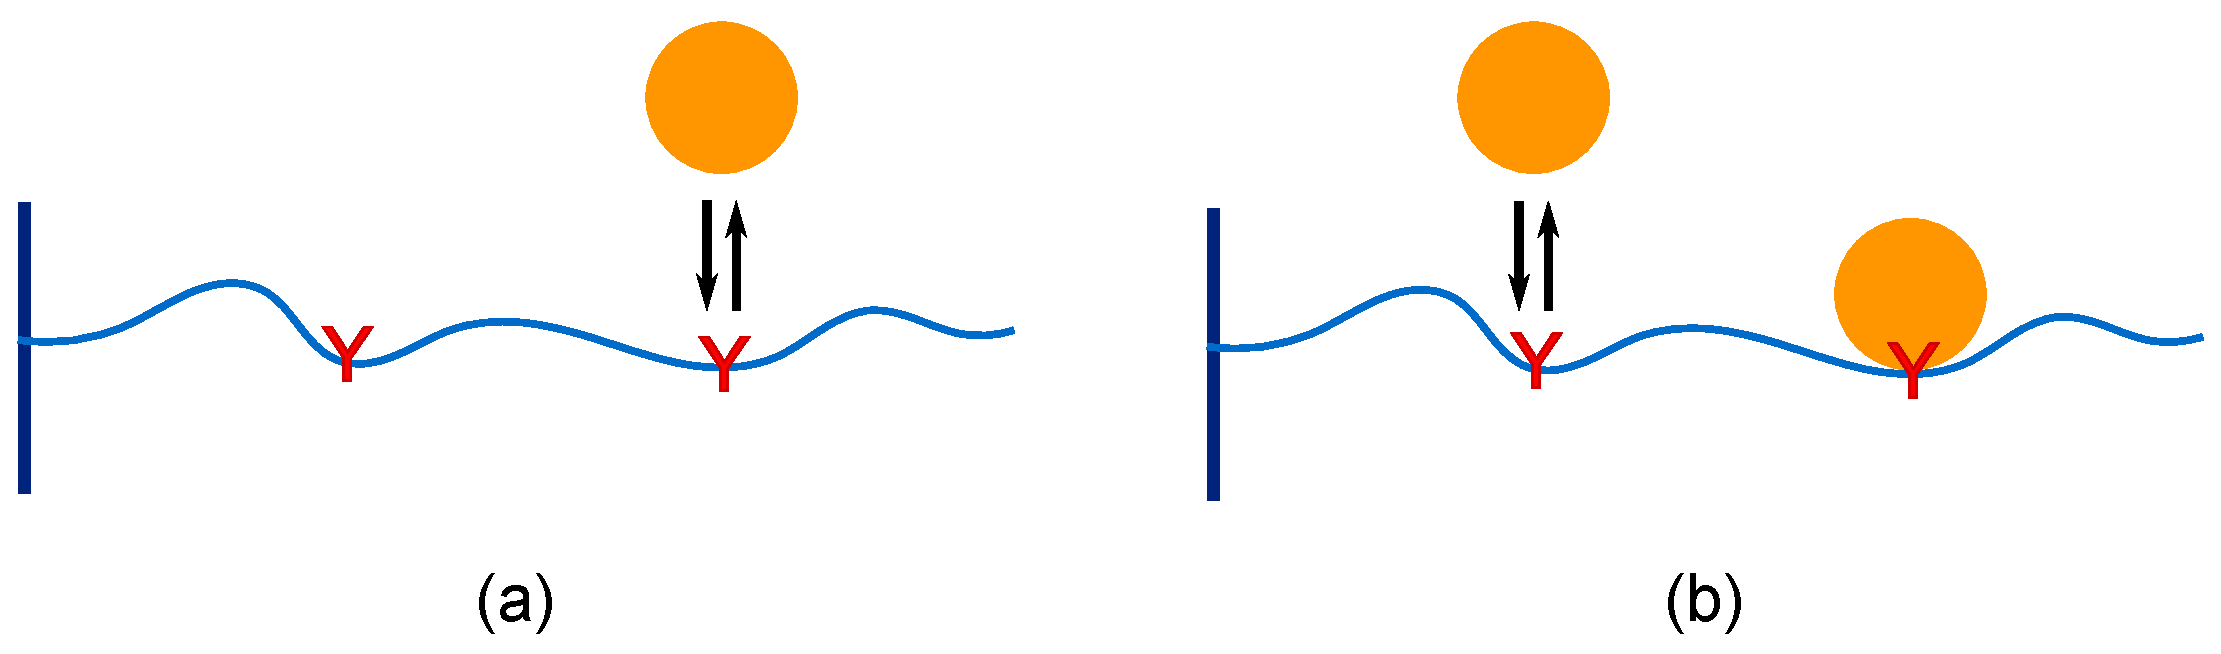
\includegraphics[width=0.8\linewidth]{ResultsFigures/SimultaneousBindingDiagram/SimultaneousBindingDiagram.eps}
    \caption{Cartoon of simultaneous binding model. Surface bound FJC prior to ligand binding (a) transitions to FJC with single bound ligand and a second ligand attempting to bind (b). \label{fig: SimBindCartoon}}
    \end{center}
\end{figure}


%%%%%%%%%%%%%%%%%%%%%%%%%%%%%%%%%%%%%%%%%%%%%%%%%%%%%%%%%%%%%%%%%%%%%%%%%%%%%%%%%%%%%%%%%%%%%%%%%%%%%
%%%%%%%%%%%%%%%%%%%%%%%%%%%%%%%%%%%%%%%%%%%%%%%%%%%%%%%%%%%%%%%%%%%%%%%%%%%%%%%%%%%%%%%%%%%%%%%%%%%%%

\subsection{Results}

\subsubsection{Negative cooperativity arises from simultaneous binding of ligands to an IDP}

% first scenario - SH2 bound, vary irL
We first explore how two ligand species binding to the same domain may influence each other's binding. We focus on a simplification of ZAP-70 and Lck molecules binding to CD3$\zeta$. We assume that each of the bound ligands is approximately the size of an SH2 domain (i.e. ZAP-70 is bound to the polymer) and we calculate the probability of a separate species binding to one of the remaining binding sites.  We investigate this for many sizes of incoming ligand, including our estimates for Lck and ZAP-70. We find simultaneous binding of multiple SH2 sized domains will cause mild to severe negative cooperativity with the binding of another ligand. Larger ligands have a harder time binding when there are multiple SH2 domains already bound. For a 4.2nm radius incoming ligand, there would be a 30 fold decrease in the probability of binding from no other bound ligands to five SH2 domains bound to the same disordered chain. Only very small ligands would be unhampered by the presence of other bound ligands. An Lck molecule, only slightly larger than an SH2 domain, would experience an approximately eight fold decrease in its ability to bind once five SH2 domains are already bound to the disordered chain. (Fig. \ref{fig: SimBindMemOnSH2})


\begin{figure}[H]
	\begin{center}
		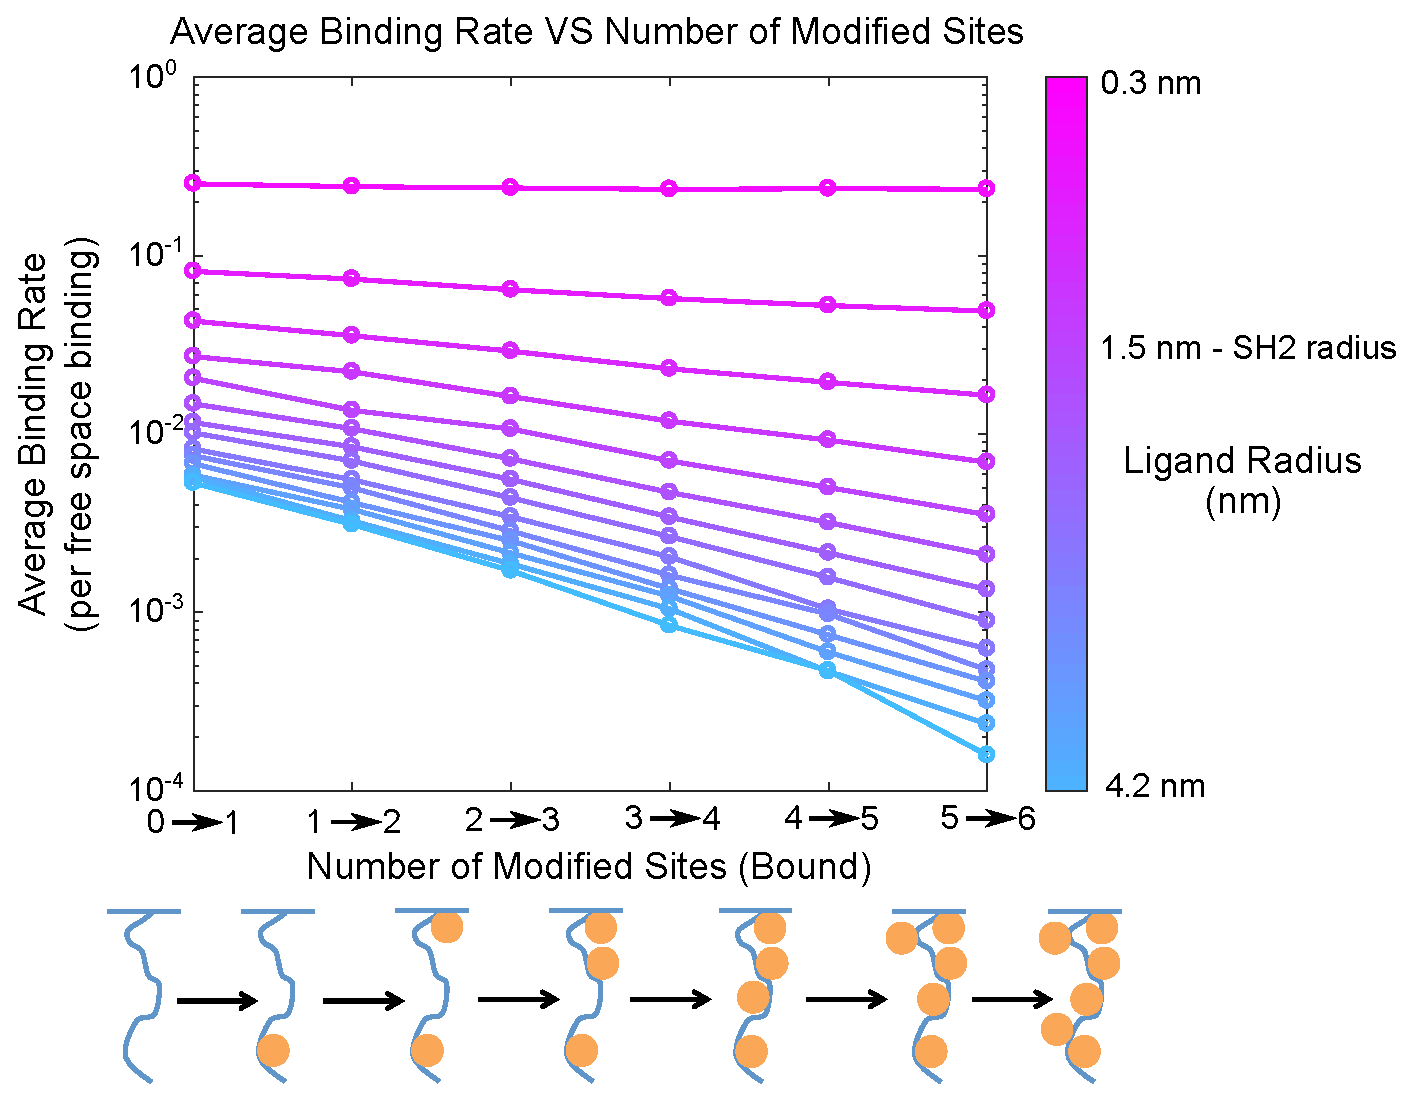
\includegraphics[width=\linewidth]{ResultsFigures/CD3ZetaMultipleBindingMembraneOn/AvgBindVSTotalPhosColorMapLabeled.eps}
		\caption{(Above) Simulated average binding rates of Lck to CD3$\zeta$ for specified number of SH2 domain sized (1.5nm radius) ligands previously bound and varying unbound ligand sizes (0.3 nm $\rightarrow$ pink, 4.2 nm $	\rightarrow$ blue). (Below) Cartoon representing a possible bound configuration series of CD3$\zeta$. \label{fig: SimBindMemOnSH2} }
	\end{center}
\end{figure}


% second scenario - equal bound and incoming radius
The second case of simultaneous binding we explore is when only one ligand species attaches to the disordered chain. We investigate how multiple bound ligands of a given size impacts another ligand of the same size binding. We see the same trend of behavior as above, but more dramatic.  Here, if we consider a ligand with radius 2.1nm, we already see a 30 fold decrease between no ligands bound and five bound. This matches intuition, since although a large bound ligand will straighten the polymer more, it will also create a much larger occluded volume making binding site accessibility much less likely.  Note that similarly, if the bound ligand size is less than that of an SH2 domain, then we actually see less negative cooperativity than when all bound ligands were SH2 domains. (Fig. \ref{fig: SimBindMemOnibEqual})

\begin{figure}[H]
	\begin{center}
		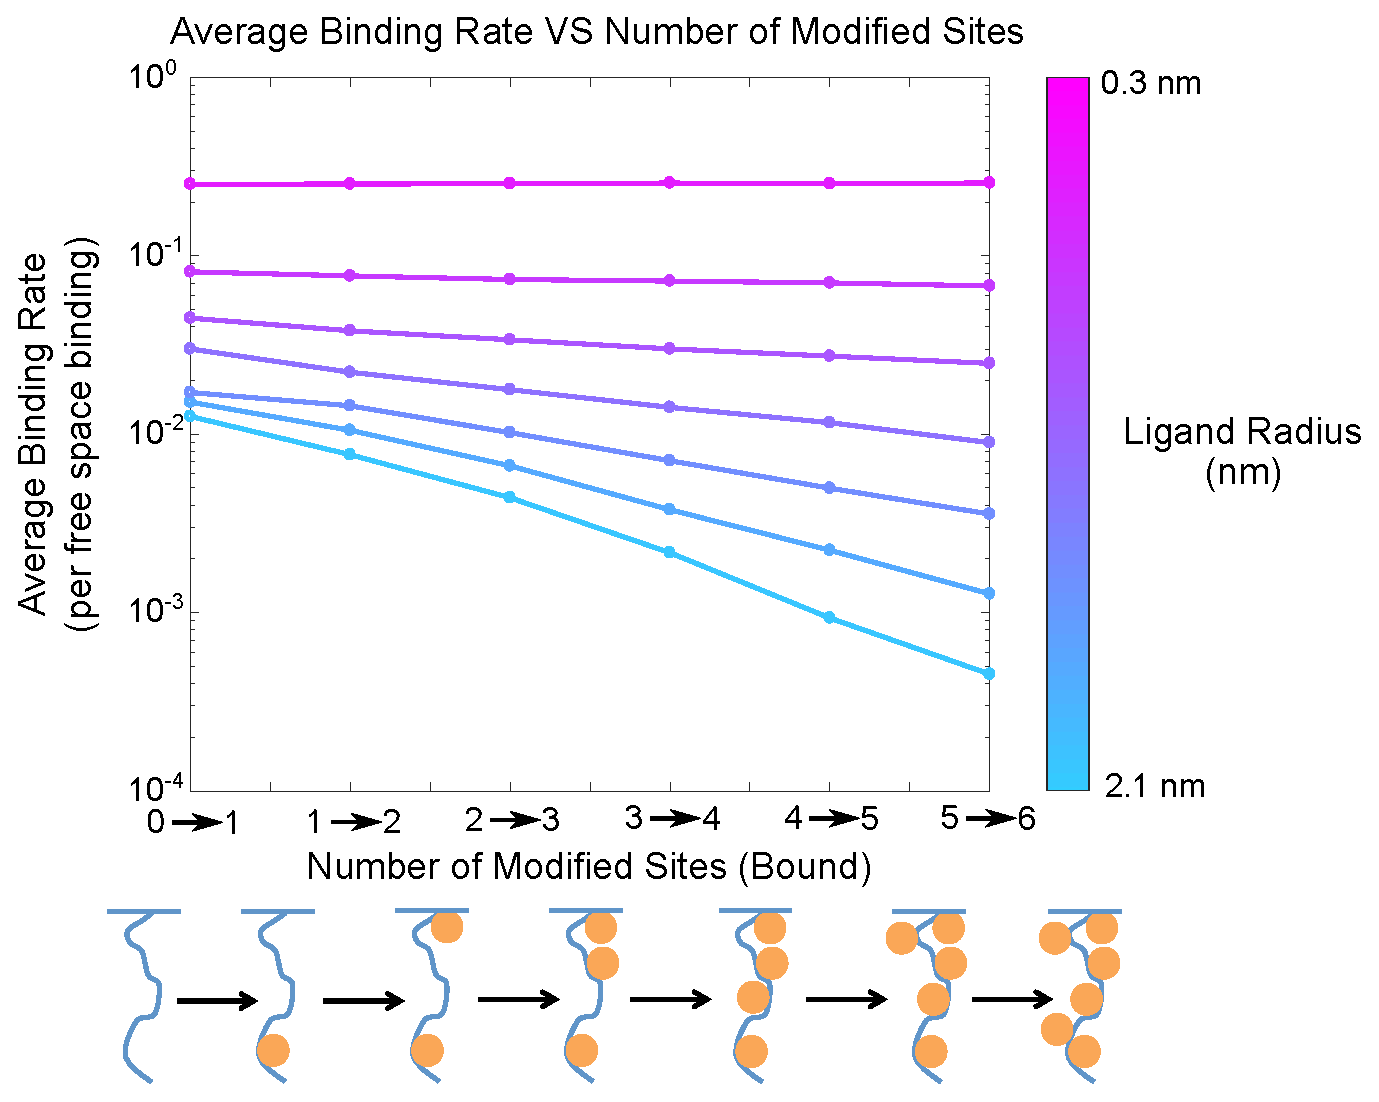
\includegraphics[width=\linewidth]{ResultsFigures/CD3ZetaMultipleBindingMembraneOn/ibEqual/AvgBindVSTotalModified.eps}
		\caption{(Above) Simulated average binding rates of Lck to CD3$\zeta$ for specified number of ligands previously bound and varying ligand sizes (0.3 nm $\rightarrow$ pink, 4.2 nm $		\rightarrow$ blue). (Below) Cartoon representing a possible bound configuration series of CD3$\zeta$. \label{fig: SimBindMemOnibEqual} }
	\end{center}
\end{figure}


\subsubsection{Future Work: Sequence of binding multiple ligands}

We obtained relative probabilities of binding for each tyrosine along the chain at each bound state.  With this information, we are able to explore whether or not there is a dominant sequence of binding events. We ran a Gillespie algorithm with six events, one for each ligand binding.  From each run, we record which sequence or 'path' of binding.  When we compile the path frequency data, it becomes clear that the first binding event is dominant.  That is to say, any path beginning by binding to the membrane distal tyrosine (6th tyrosine), will occur more often than any path beginning with the membrane proximal tyrosine. 

For simplicity, we consider only the paths membrane proximal to membrane distal (123456) and distal to proximal (654321). We see that when a membrane is present, the probability of binding distal to proximal is much higher than that of phosphorylating proximal to distal. This phenomenon is easily explained by the presence of a membrane. The membrane proximal tyrosine has a smaller range of space it may occupy than the distal tyrosine.  Therefore, it is more likely to be close to the membrane in a configuration.  Since the ligand cannot penetrate the membrane, tyrosines closer to the membrane have a higher probability of being effectively sheltered from ligand binding. This makes the distal to proximal path much more likely. 

The preference for distal to proximal binding is enhanced by increasing ligand size.  Larger ligands remain able to bind the membrane distal tyrosine with similar probability but will have a lower probability of binding tyrosines close to the membrane. When we simulate CD3$\zeta$ without a membrane, this preference is eliminated.  Note that unlike with the local structuring model, a strict comparison of distal to proximal vs proximal to distal binding does not indicate a preference based on uneven spacing of tyrosines and in fact both of these paths are less likely than if all paths were equally probable. Although the most likely tyrosine to be bound is still the distal tyrosine, there is not a strong preference for the distal to proximal sequence because perfectly sequential binding is unlikely.  Each bound ligand is more likely to sterically occlude a neighboring tyrosine than one further away.  Therefore, if the distal tyrosine is the first bound, the next most likely to be bound is not its neighbor.

We are soon going to introduce a ranking system for the paths in order to do a full analysis of all possible paths. We look to answer if, for simultaneous binding, there a single path or group of paths that stand out as most likely. 

\begin{figure}[H]
	\begin{center}
		\begin{subfigure}{0.3\linewidth}
			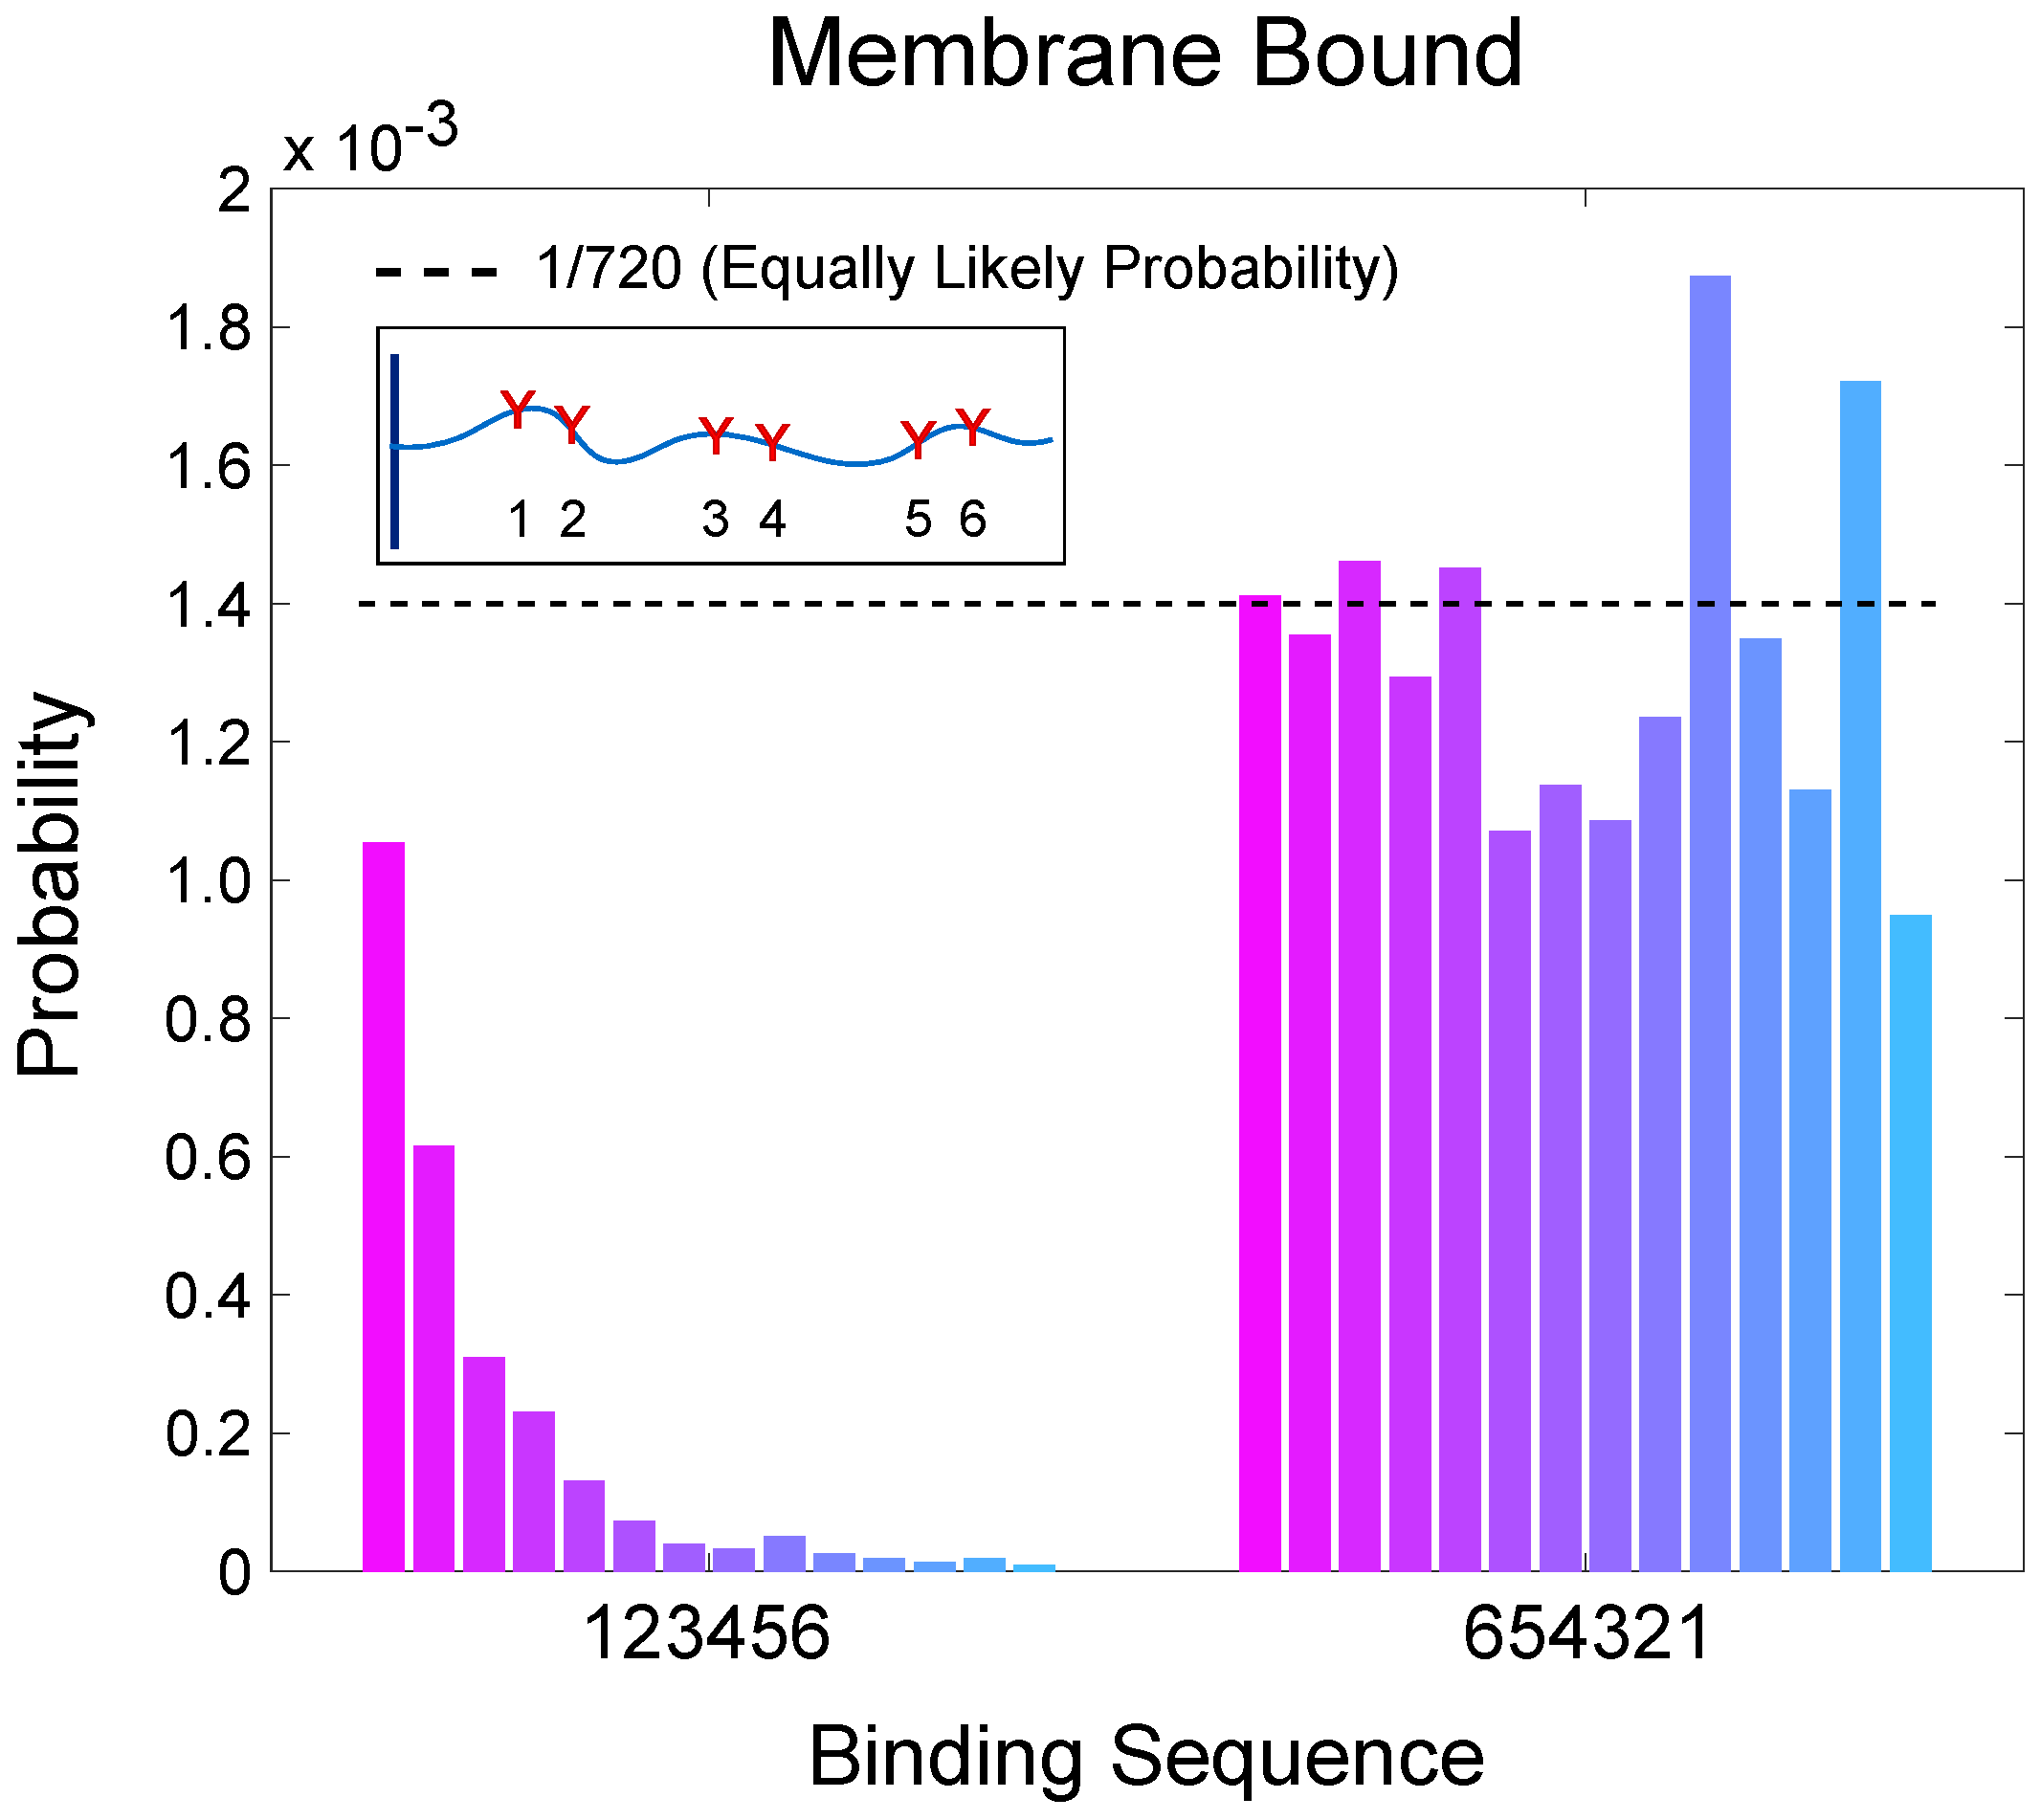
\includegraphics[width=\linewidth]{ResultsFigures/MultipleSequentialBinding/MemOn/ProbVSSequence.eps}
			\caption{}
		\end{subfigure}
		\begin{subfigure}{0.3\linewidth}
			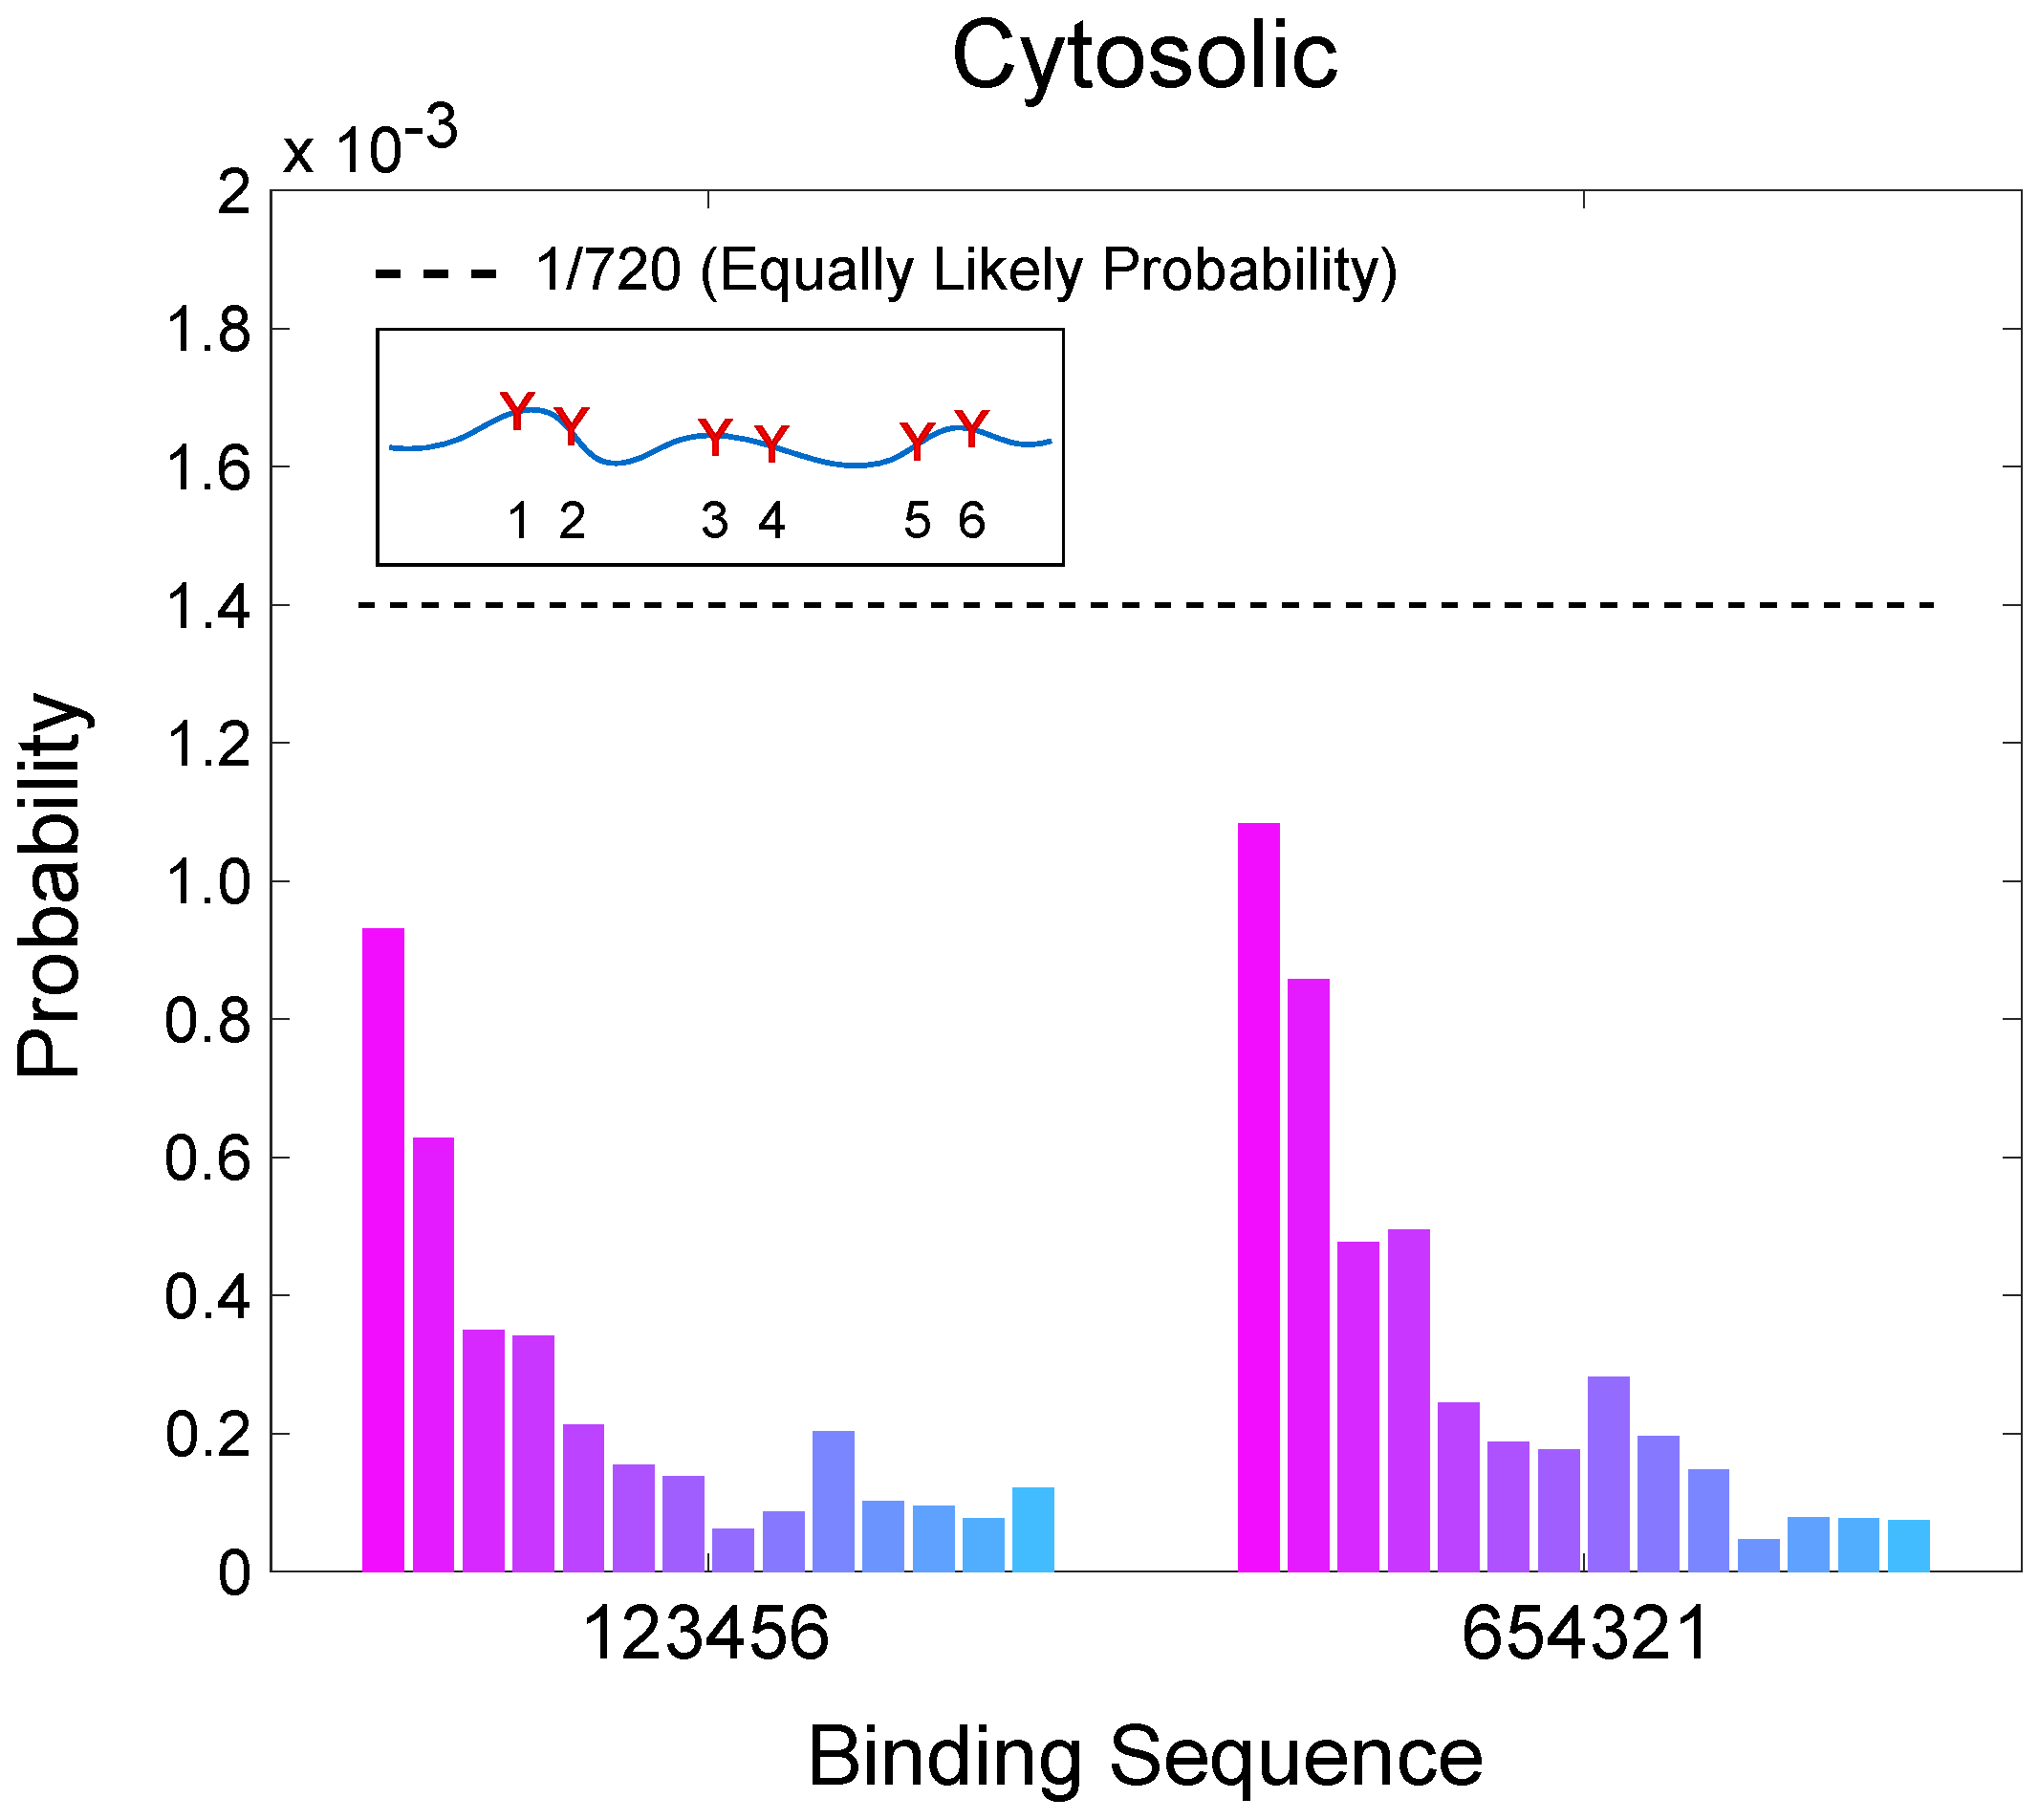
\includegraphics[width=\linewidth]{ResultsFigures/MultipleSequentialBinding/MemOff/ProbVSSequence.eps}
			\caption{}
		\end{subfigure}
		\begin{subfigure}{0.3\linewidth}
			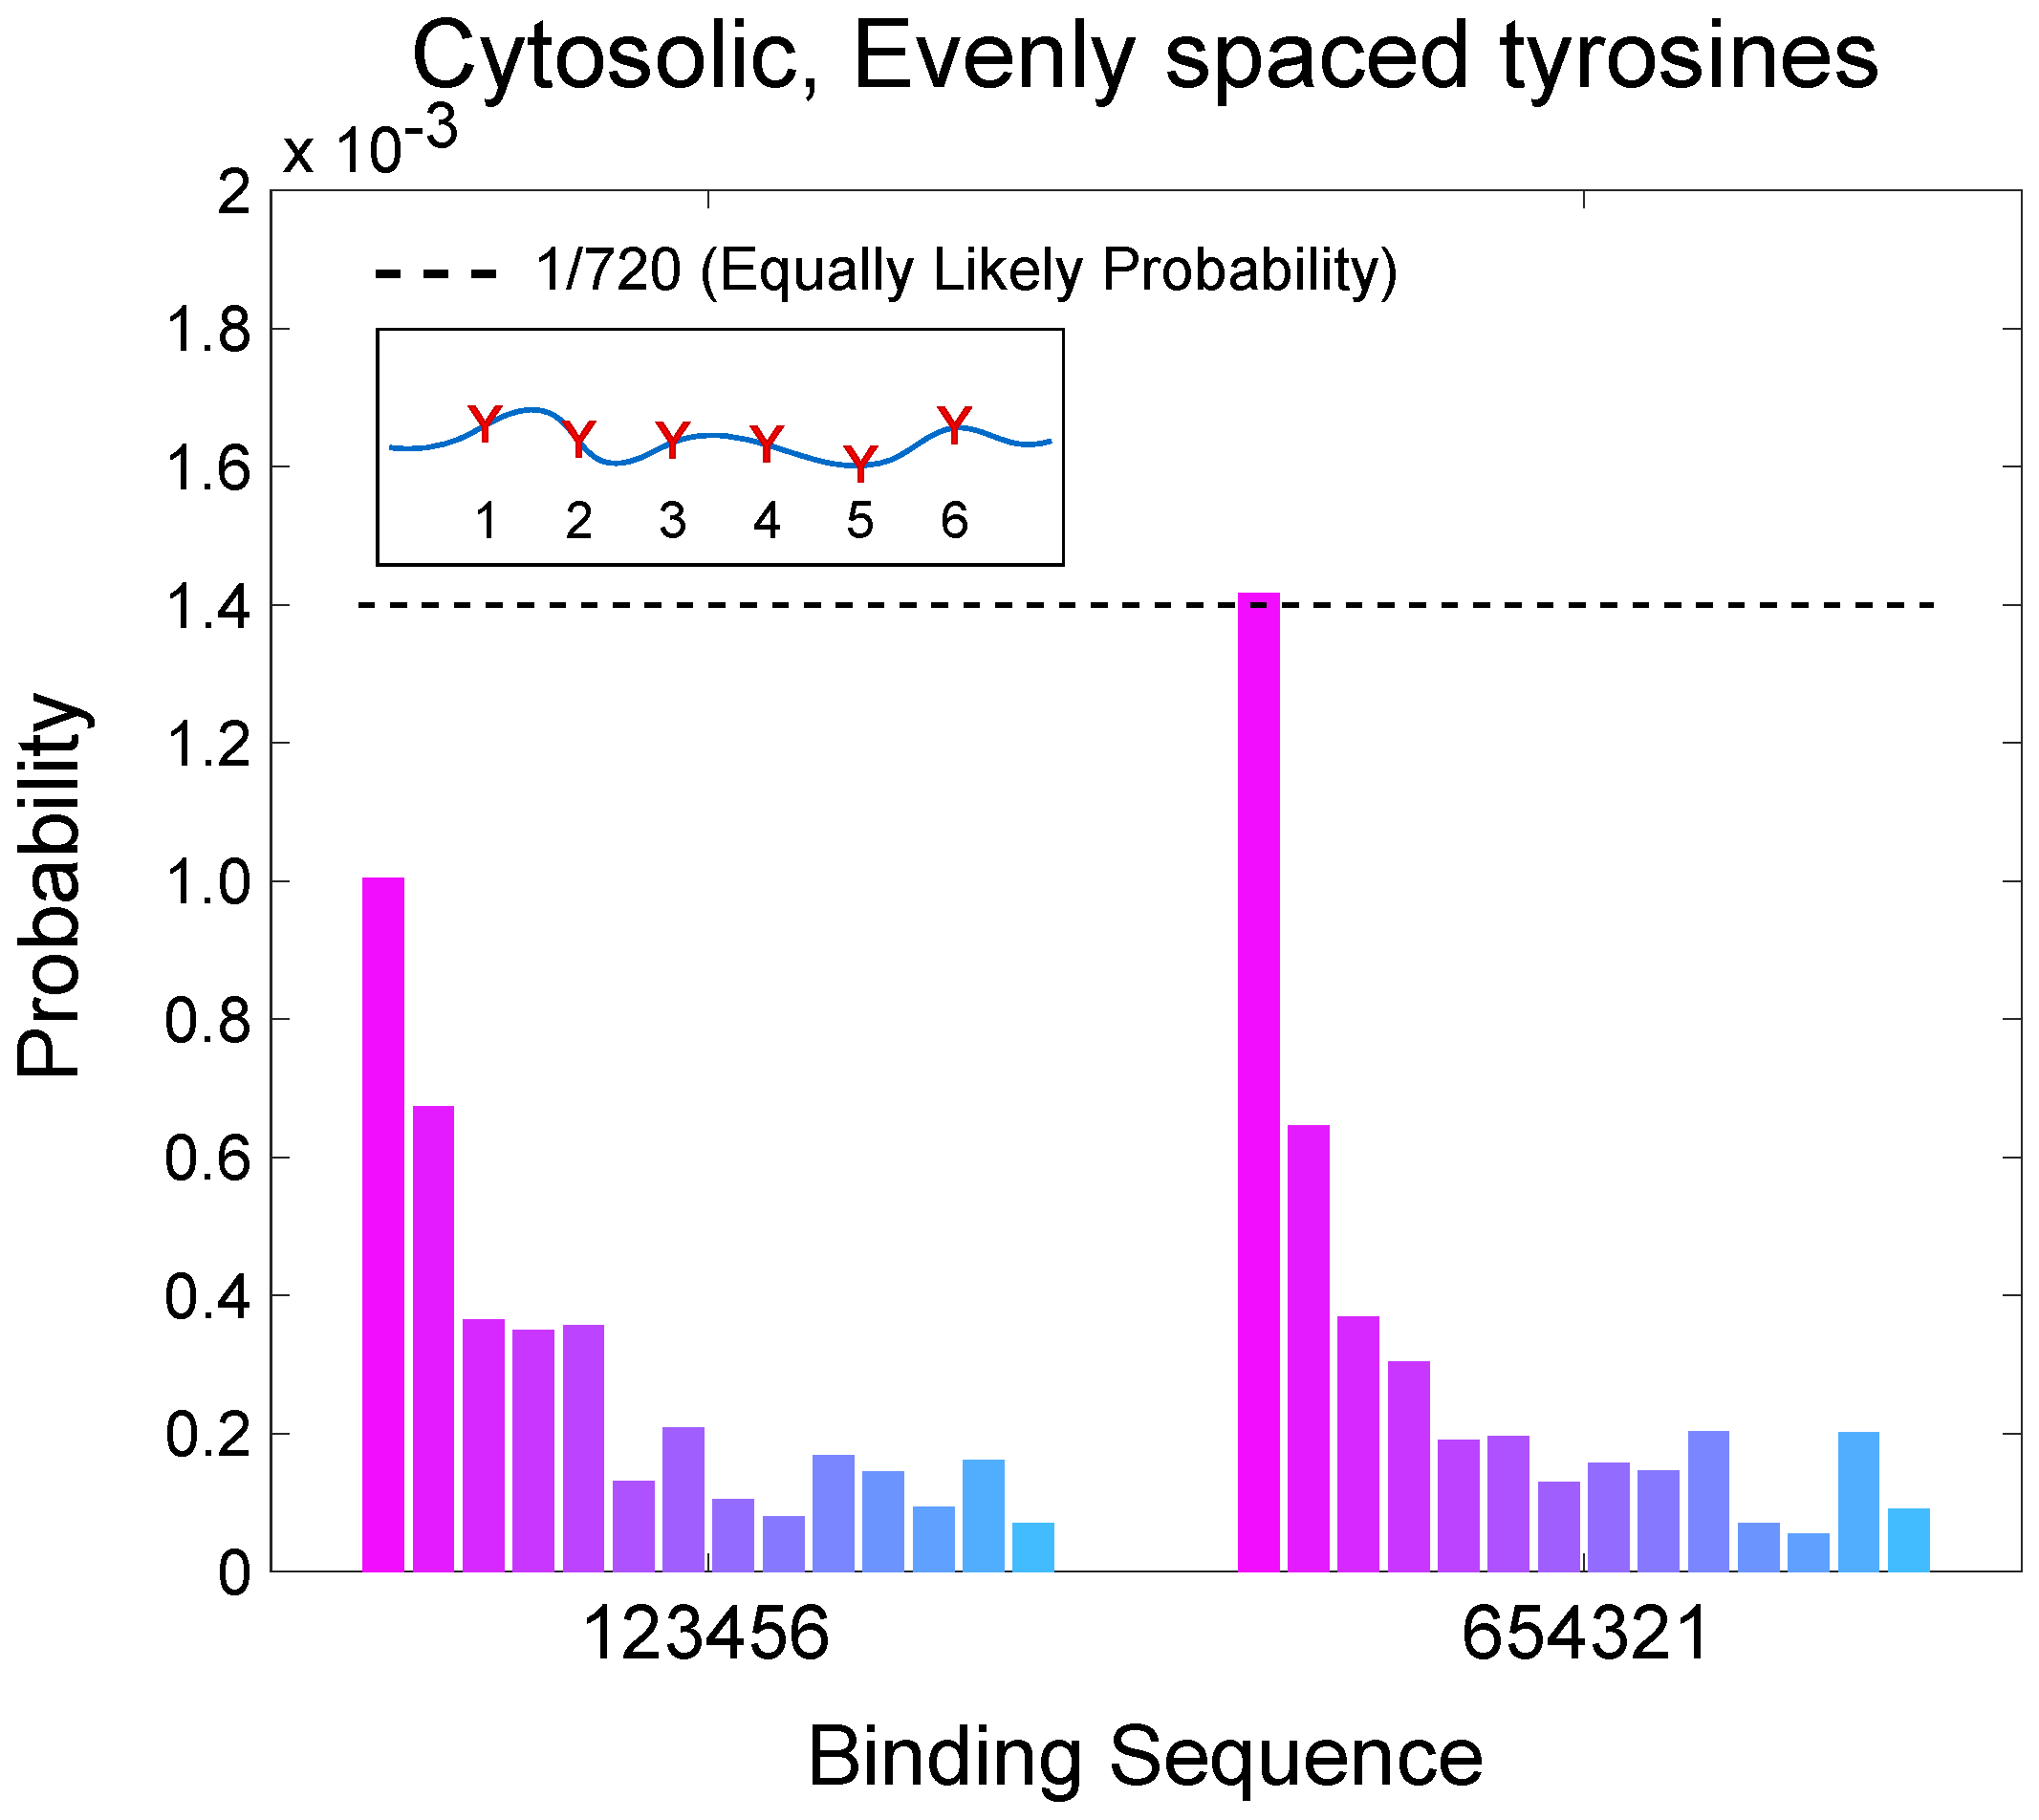
\includegraphics[width=\linewidth]{ResultsFigures/MultipleSequentialBinding/EvenSites/ProbVSSequence.eps}
			\caption{}
		\end{subfigure}
	\end{center}
	\caption{Probability of ligand binding membrane proximal to distal (123456) compared with distal to proximal (654321). Equally likely probability of all paths indicated with black, dotted line. (a) CD3$\zeta$ parameters, with membrane. (b) CD3$\zeta$ parameters, without membrane. (c) CD3$\zeta$ length, evenly spaced tyrosine locations, without membrane.}
\end{figure}

\subsubsection{Future Work: Multiple chains towards a full model of a T cell receptor signalosome}

There is work showing that six ZAP-70 molecules bind to the disordered proteins of the T Cell Receptor on average.  \cite{ODonoghue2013} We want to eventually report an equilibrium value for the number of molecules able to bind to a CD3$\zeta$ chain. We will also expand our model to include all of the domains of the receptor. This will allow us to test if steric effects are sufficient to explain why only six ZAP-70 molecules would bind to the receptor simultaneously.  When all of the chains are included in the simulation, each chain will be able to explicitly occlude binding sites on other domains. Experimental work on CD3$\zeta$ and other receptors is often completed using dimers. \cite{Mukhopadhyay2016} \cite{Dobbins2016} Simulating multiple domains will allow us to better relate our results to the experimental results. 

Eventually, we would like to include co-receptors of TCR in our model. This will help expand our understanding of the TCR network, in particular elucidating why co-receptors are necessary for full T cell signaling, e.g. CD4 and CD8. There is evidence that Lck is associated with membrane-bound proteins CD4 and CD8 \cite{Barber1989},\cite{Veillette1988},\cite{Rudd1988}. There is also evidence that the phosphatases involved with TCR triggering, CD45 and CD148, are also membrane bound. \cite{Davis2006} These changes to the model will give finer detail to our understanding of the dynamics of reversible phosphorylation of the CD3$\zeta$ chain.




%%%%%%%%%%%%%%%%%%%%%%%%%%%%%%%%%%%%%%%%%%%%%%%%%%%%%%%%%%%%%%%%%%%%%%%%%%%%%%%%%%%%%%%%%%%%%%%%%%%%%
%%%%%%%%%%%%%%%%%%%%%%%%%%%%%%%%%%%%%%%%%%%%%%%%%%%%%%%%%%%%%%%%%%%%%%%%%%%%%%%%%%%%%%%%%%%%%%%%%%%%%
\subsection{Discussion}

An Lck molecule, only slightly larger than an SH2 domain, would experience an approximately eight fold decrease in its ability to bind once five SH2 domains are already bound to the disordered chain. This suggests the CD3$\zeta$ chain is mostly phosphorylated before ZAP-70 begins to attach or that phosphorylation by Lck slows down when ZAP-70 attaches.  In the second case, this could lead to phosphorylation needing to occur via another mechanism, for instance via the kinase domain of ZAP-70 itself.  

Simultaneous binding of ligands leads to negative cooperativity. This endows signaling systems with two features: high turnover of ligands even in high ligand concentration (which might be advantageous if ligands are involved in other reactions), and constant signaling activity in low ligand concentration. Similarly, this might reduce the impact of inhibitors, requiring much higher concentrations of inhibitor to completely turn off signaling.



%%%%%%%%%%%%%%%%%%%%%%%%%%%%%%%%%%%%%%%%%%%%%%%%%%%
\end{document}
%%%%%%%%%%%%%%%%%%%%%%%%%%%%%%%%%%%%%%%%%%%%%%%%%%%





